Compared to most engineering projects, the present work is profiled as a distinct, highly conceptual idea. Investment costs are practically null. There is no equipment required other than a computer or cluster to run the PGD. In essence, rather than an installation, the project details a potentially beneficial service to customers, prosumers, generators, and the DSO. A Business model Canvas is depicted in Figure \ref{fig:canvas1} to put into perspective the business side of the project. 



\begin{figure}[!htb]
\centering
\def\layersep{3em}
\def\layerwidth{14.5cm}
\makebox[\textwidth][c]{
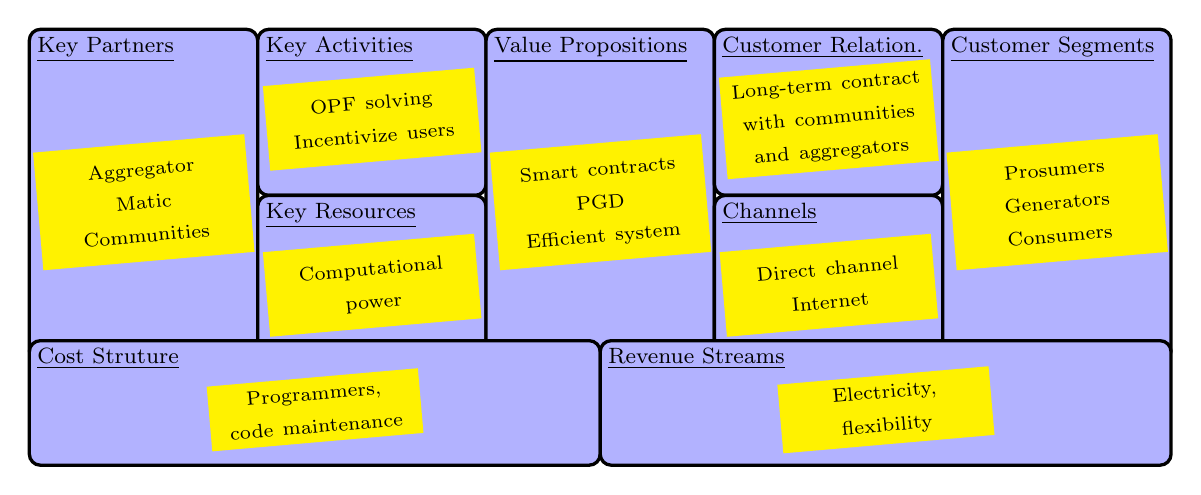
\begin{tikzpicture}[
% Here are defined the bocks and post-its parameters (e.g. shape, color and rotation)
bloc/.style={
rectangle, rounded corners,
draw=black, very thick, inner sep=0,
fill=blue!30 },
bloc1/.style={
bloc,
minimum width = \layerwidth/5,
minimum height= 4*\layersep },
bloc2/.style={
bloc,
minimum width=\layerwidth/5,
minimum height=2*\layersep },
bloc3/.style={
bloc,
text width=\layerwidth/2,
minimum height=1.5*\layersep },
postit/.style={
rectangle, text width=\layerwidth/5.9,
rotate around={5:(1,0)},
text centered, fill=yellow },
title/.style={
anchor=north west },
]

%%%%%%%%%%%%%%%%%%%%%%%%
%%% DRAW THE CANVAS
%%%%%%%%%%%%%%%%%%%%%%%%

% The 7 top blocks

% We start drawing the top left bloc here
% 1st, the block, then the title, then the post-it
\node[bloc1] (b0) at (0*\layerwidth/10,4*\layersep) {};
\node[title] at (b0.north west) {\underline{\footnotesize Key Partners}};
% \node[postit] at (b0.center) {Angel investors};
\node[postit] at (b0.center) { \begin{tabular}{c} \scriptsize{Aggregator} \\ \scriptsize{Matic} \\ \scriptsize{Communities}\end{tabular} };

\node[bloc2] (b1) at (2*\layerwidth/10,5*\layersep) {};
\node[title] at (b1.north west) {\underline{\footnotesize Key Activities}};
\node[postit] at (b1.center) { \begin{tabular}{c} \scriptsize{OPF solving} \\ \scriptsize{Incentivize users} \end{tabular} };

\node[bloc2] (b2) at (2*\layerwidth/10,3*\layersep) {};
\node[title] at (b2.north west) {\underline{\footnotesize Key Resources}};
\node[postit] at (b2.center) { \begin{tabular}{c} \scriptsize{Computational} \\ \scriptsize {power} \end{tabular} };

\node[bloc1] (b3) at (4*\layerwidth/10,4*\layersep) {};
\node[title] at (b3.north west) {\underline{\footnotesize Value Propositions}};
\node[postit] at (b3.center) { \begin{tabular}{c} \scriptsize{Smart contracts} \\ \scriptsize{PGD} \\ \scriptsize{Efficient system} \end{tabular} };

\node[bloc2] (b4) at (6*\layerwidth/10,5*\layersep) {};
\node[title] at (b4.north west) {\underline{\footnotesize Customer Relation.}};
\node[postit] at (b4.center) {\scriptsize{Long-term contract} \\ \scriptsize{with communities and aggregators} };

\node[bloc2] (b5) at (6*\layerwidth/10,3*\layersep) {};
\node[title] at (b5.north west) {\underline{\footnotesize Channels}};
\node[postit] at (b5.center) { \begin{tabular}{c} \scriptsize{Direct channel} \\ \scriptsize{Internet} \end{tabular} }; ;

\node[bloc1] (b6) at (8*\layerwidth/10,4*\layersep) {};
\node[title] at (b6.north west) {\underline{\footnotesize Customer Segments}};
\node[postit] at (b6.center) { \begin{tabular}{c} \scriptsize{Prosumers} \\ \scriptsize{Generators} \\ \scriptsize{Consumers} \end{tabular} };

%%%% The 2 bottom blocks
\node[bloc3] (b7) at (1.5*\layerwidth/10,1.5*\layersep) {};
\node[title] at (b7.north west) {\underline{\footnotesize Cost Struture}};
\node[postit] at (b7.center) {\scriptsize{Programmers, code maintenance}};

\node[bloc3] (b8) at (6.5*\layerwidth/10,1.5*\layersep) {};
\node[title] at (b8.north west) {\underline{\footnotesize Revenue Streams}};
\node[postit] at (b8.center) {\scriptsize{Electricity, flexibility}};

\end{tikzpicture}
}
\caption{Business model Canvas for the combination of the PGD and smart contracts}
\label{fig:canvas1}
\end{figure}
The project propositions revolve around the idea of obtaining the optimal operating point and embedding this information in the blockchain, with a special focus on the efficiency and computational effort required. What makes this project stand apart is not only the combination of both ideas but also the scalability it offers. If the number of buses in the system grows, the PGD would still be able to solve the power flow relatively fast, at least much faster than traditional methods. Besides, even if the amount of transactions increases dramatically, the overall absolute cost would remain low, and the speed of the transaction would be kept at around 2 seconds. 

The DSO has to establish partnerships with communities, rather than individual household customers. It is not viable to solve an OPF at the individual level, as the distribution grid becomes too complex to be modeled in detail. Thus, in order to reduce the simplicity, it is convenient to aggregate users in communities or \textit{concelhos}. In a future electricity market, the aggregator might become the stakeholder responsible for doing precisely this. Therefore, long-term commercial relationships have to be established between the DSO and the communities or aggregators.

Broadly speaking, the customer segment involves all users connected to the grid. The PGD can handle theoretically any number of dimensions, which means that there could be one dimension attributed to every bus. This would be responsible for scaling the powers, for instance. Consequently, in practical terms, it would not make any difference if the user is a consumer, generator, or prosumer. In this context where the DSO acts simultaneously as a retailer, both power and flexibility are exchanged with the user. The DSO then rewards users in a way that incentivizes the common good. Both parties are expected to benefit from it. Users may be able to pay less for their electricity, generate revenue from selling it, and be compensated for the offered flexibility. The DSO could reduce the total losses of the system, and minimize the power exchanged with the TSO. 

Regarding the strengths, weaknesses, opportunities and threats of the project, they are illustrated in Figure \ref{fig:swot} in the form of a SWOT analysis. 

% communications :smart meters



\begin{figure}[!htb] \centering
\begin{tikzpicture}[
    any/.style={minimum width=3.5cm,minimum height=3.5cm,%
                 text width=3.5cm,align=center,outer sep=0pt},
    header/.style={any,minimum height=1cm,fill=black!10},
    leftcol/.style={header,rotate=90},
    mycolor/.style={fill=#1, text=#1!60!black}
]

\matrix (SWOT) [matrix of nodes,nodes={any,anchor=center},%
                column sep=-\pgflinewidth,%
                row sep=-\pgflinewidth,%
                row 1/.style={nodes=header},%
                column 1/.style={nodes=leftcol},
                inner sep=0pt]  
{
          &|[fill=helpful]| {\texta} & |[fill=harmful]| {\textb} \\
|[fill=internal]| {\textcn} & |[mycolor=S]| \back{S} & |[mycolor=W]| \back{W} \\
|[fill=external]| {\textdn} & |[mycolor=O]| \back{O} & |[mycolor=T]| \back{T} \\
};

\node[any, anchor=center] at (SWOT-2-2) {Secure energy transactions\\ {.}\\ Fast OPF calculation};
\node[any, anchor=center] at (SWOT-2-3) {Agreement between prosumers and DSO\\ {.}\\ Idea stage};
\node[any, anchor=center] at (SWOT-3-2) {Enhance prosumers' participation\\ {.}\\ Minimize losses};
\node[any, anchor=center] at (SWOT-3-3) {Current market structure\\ {.} \\ Unwillingness to participate};

\end{tikzpicture}
\caption{SWOT for combination of the PGD and smart contracts}
\label{fig:swot}
\end{figure}
The difficulty of implementing the project is found in the necessity of establishing solid agreements with users. Users have to identify their participation as valuable, not only for their economical gains but also to sustain an optimal grid operation. In addition to that, the current market structure is likely to complicate the implementation of the project. Since users have contracted a particular retailer, communication should be established between the DSO and the retailer, and subsequently between the retailer and the users. This overcomplicates the approach selected in the project, where the retailer is dismissed, or rather, integrated into the DSO. Changes in regulation could promote the evolution of the electricity market towards the vision depicted in this project. 

Regarding the economic part, a reduction of just 0.1\% in the losses of the system (smaller by an order of magnitude compared to the amount found in the case study) is likely to be achieved. This represents a quite significant saving of energy if the numbers are scaled up. For instance, Portugal had an energy generation of 56129 GWh and an energy consumption of 48035 GWh back in 2018 \cite{edpp}. This way, a 0.1\% improvement in the overall efficiency of the system would imply a saving of 65.51 GWh. Assuming a price of 57 \euro/MWh, which corresponds to the wholesale electricity market price of Iberia in 2018, the total saving represents 3.73 M\euro \ \cite{edpr}. 

There are only two costs associated with the project. One has to do with the transactions and is represented by the so-called gas fees. Although extremely small, these could be paid between the DSO and the users. The second cost is the engineering team. It would be in charge of ensuring the correct real-time operation of the PGD and setting the platform to interact with the user. It is hard to determine beforehand this cost. But overall, the message we want to transmit is that there is huge economic potential. 

